\section{Introduction}\label{sec:intro}
Cut cell meshes to solve hyperbolic problems 
are increasingly prevalent due to the ease 
of grid generation for complicated geometries. 
However the {\em small cell} problem is still an active area of research, and
a completely satisfactory solution has not yet been found.
The small cell problem can be explained as follows: explicit
finite volume schemes typically need to take a time step 
that is proportional to the mesh width in order to satisfy a CFL constraint for
stability. However cut cells can have volumes that are arbitrarily
smaller than the regular cells that would otherwise determine the stable time
step. Special algorthms are needed to prevent this restriction.

The most commonly used stabilization algorithm is called flux
redistribution \cite{chern:colella,vof:colella}. The main idea is illustrated below in two space
dimensions, for ease of notation.
The essential idea is to compute the 
flux update for a cut cell $i,j$ with volume $V_{i,j} < V_{\mbox{\em full}}$,
\begin{eqnarray*}
V_{i,j} Q_{i,j} ^{n+1} & = V_{i,j} Q_{i,j}^n  +  \Delta t \, \Sigma_k F_k \cdot l_{k}\\
                   & = V_{i,j} Q_{i,j}^n  +  \delta  M 
\end{eqnarray*}
Here, $V_{\mbox{\em full}}$ is the volume of a full uncut cell.
Instead of using the entire amount of the update in cell ${i,j}$, 
the cut cell only uses a fraction $\eta$ of it.  If the fraction $\eta$
is proportional to the cell's volume
fraction $V_{i,j}/V_{\mbox{\em full}}$, the update should be stable. 
To maintain conservation, the rest of the update ($1-\eta)\delta M$
is given to the cell's neighbors.  
There are more recent additional steps that make the distribution 
more robust and accurate. For example, the difference between a stable
non-conservative update and the conservative update is what is
redistributed (see \cite{vof:colella} for details).
Flux redistribution has already been implemented for three dimensional
calculations due to its simplicity. However it is only first order
accurate at the cut cells.

Cell merging is most frequently the first idea people 
think of. It is conceptually simple, but 
we are not aware of any production codes that implement this in a fully
general, robust manner for complicated engineering geometries. 
The $h$-box method \cite{mjb-hel-rjl:hbox2,mjb-hel:hboxsimple}
is a second order accurate method at the cut cells. It extends the 
domain of dependence for the fluxes around a small cell in a 
special way that maintains stability by means of a cancellation
property. It  has not been extended to
three dimensions due to its complexity. 

A newer variation of cell merging is called cell linking \cite{cecereGiacomazzi,
KirkpatrickEtAl:2003, HuKhooAdamsHuang:2006,Chung et al} 
This has simpler data structures and maintain the original grid. 
Many of these references tackle incompressible flow; some also include
three dimensional examples. Several references use a staggered mesh. 

In \cite{BalajiMenon:2016}, the authors improve the accuracy of cell linking,
with a third order accurate approach for viscous flow,  and fourth order for 
inviscid flow. 
Their version of cell linking uses a cluster of cells,
while still maintaining each cell in the mesh.  A high order
polynomial is fit to the cluster, and replaces the solution values in the
individual cells.  Our algorithm has a similar spirit to this, though the
details are very different. 

In \cite{shws:2011}, the authors make
some improvements to flux redistribution for viscous flow in moving
geometries. They introduce a
smooth cutoff function of cell size for when it is applied. They also
use a non-uniform weighting in the gradient stencil to avoid abrupt
changes, which can lead to oscillations in the solution. This is
especially important for moving geometries.

In \cite{May-Berger:JSC}, an implicit scheme was developed to
handle stability of the cut cells, and was combined with an 
explicit method for the full cells. In this work we will focus on 
two explicit methods, and make modification necessary for their accuracy 
on cut cells.
Other approaches that have been proposed in the literature include
interpolation-based procedures, such as the mirror-cell method by Forrer
and Jeltsch \cite{article:FoJe98}, and a related ghost-fluid method by
Dadone and Grossman \cite{DadoneGrossman}.
There are also approaches based on finite difference schemes
\cite{SjogreenPetersson,MarcoBjorn}
and kinetic schemes \cite{Oksuzoglu:thesis,KeenKarni}.
However, since we are interested in methods
that preserve conservation we do not explore these alternatives further.

In this paper we propose a framework for a stabilization algorithm in
the spirit of flux redistribution (henceforth FRD). 
As with FRD, it is applied as a postprocessing
step, and is simple to implement. Cell updates on all cells are performed
with a fixedd $\Delta t$ using whatever the base finite volume scheme is, followed by a 
postprocessing step based on the
conserved state variables, not on the fluxes.
Hence we call it {\em state redistribution} (SRD).


To set the stage, notice that cell merging itself can
be rewritten as a postprocessing step.
\commentout{
To take one step to update a finite volume approximation to
$u_t + u_x = 0$ we do the following:
\begin{itemize}
\setlength\itemsep{.2in}
\item
{\bf Finite Volume Step}\\
Take the usual finite volume step with fixed, regular  $\Delta t$ on all cells 
including the small cell:
\begin{equation}
\bar{u}_j = u_j^n - \frac{\Delta t}{h_j} \; (f_{j+1/2} - f_{j-1/2} ), 
\quad \forall j.
\label{eqn:fvupdate}
\end{equation}

\item
{\bf {\em Temporarily} Create Merged Cell}\\
Temporarily create the {\em merged} cell $\overline{u_M}$ consisting of the small cell $u_j$ and one
or both of its neighbors so that it the merged cell is of sufficient
size (to be discussed later).  For simplicity here we will merge 
only with the neighbor on the right,
\begin{equation}
\widehat{q_M} =  \frac{ h_k \bar{u}_k + h_{k+1} \bar{u}_{k+1} } {h_k +
h_{k+1}} .
\label{eqn:mergestep}
\end{equation}

\item
{\bf Compute Merge Cell Gradient }\\
There are several ways to do this. 
Two simple possibilities are 
\begin{equation}
\nabla \widehat{u_M} = \frac{\bar{u}_{k+2} - \bar{u}_{k-1}} {x_{k+2}-x_{k-1}}
\label{eqn:gradLim1}
\end{equation}
which does not use the merged cell,
or
\begin{equation}
\nabla \widehat{u_M} = \frac{\bar{q}_{k+2} - \widehat{u_{M}}} {x_{k+2}-x_{M}}
\label{eqn:gradLim2}
\end{equation}
which uses the merged cell, and $x_M$ is the centroid of the merged
cell.
The choice of gradient stencil will be studied later in section \ref{sec:srdAlg}.

%Other more accurate alternatives exist, not all of which are stable.
%It would be better to use smaller stencils, perhaps including $u_{k+1}$
%or $\overline{u_M}$ itself.

\item
{\bf Redistribute Merged State to Cells Comprising Merged cell }\\
Replace the provisional values computed in the cells comprising the
merged cell with the merged solution reconstructed to the cell
centroids:
\begin{equation}
\begin{split}
u_k^{n+1} &= \widehat{u_M} +  (x_k - x_M) \nabla \widehat{u_M}\\
u_{k+1}^{n+1} &= \widehat{u_M} +  (x_{k+1} - x_M) \nabla \widehat{u_M}
\end{split}
\end{equation}
\end{itemize}
}
First  update cells $k$ and $k+1$, shown in Figure \ref{fig:modelProblem1},  using a 
standard finite volume scheme on all cells:
\begin{equation}
\bar{u}_j = u_j^n - \frac{\Delta t}{h_j} \; (f_{j+1/2} - f_{j-1/2} ), 
\quad \forall j.
\label{eqn:fvupdate}
\end{equation}
Next form the merged cell
\begin{equation}
\widehat{q_M} =  \frac{ h_k \bar{u}_k + h_{k+1} \bar{u}_{k+1} } {h_k +
h_{k+1}} .
\label{eqn:mergestep}
\end{equation}
which works out to
\begin{equation}
\widehat{q_M} = \widehat{q_M}^n - 
\frac{\Delta t}{h_k + h_{k+1}} (f_{k+3/2} - f_{k-1/2})
\end{equation}

\begin{figure}
\begin{center}
%\vspace*{-.5in}
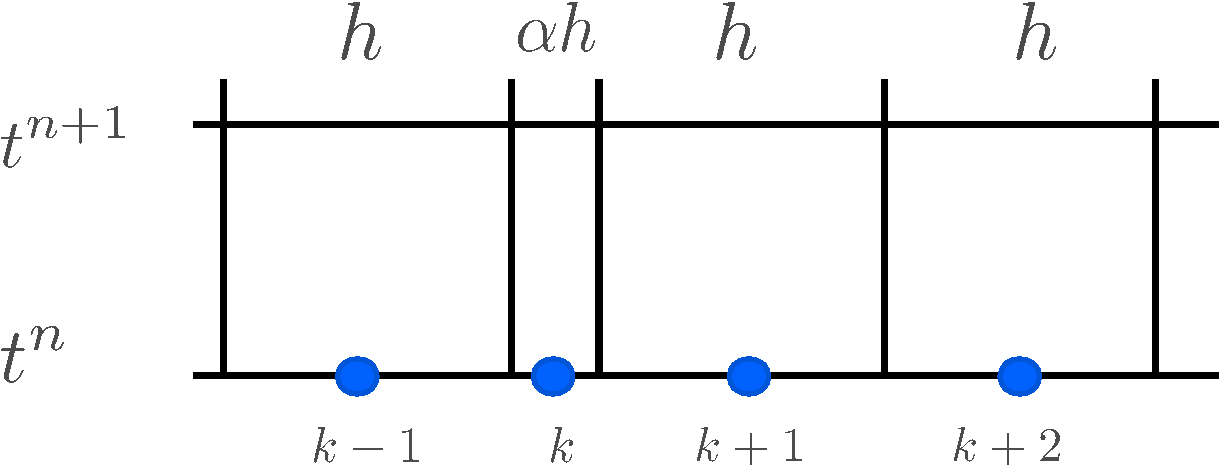
\includegraphics[height=1.3in]{figs/1dfig.pdf}
\caption{\sf Notation for model problem in one space dimension. The small
cell has size $\alpha h$ in a mesh with regular mesh width $h$.}
\label{fig:modelProblem1}
\end{center}
\end{figure}


For the simplest first order version, we simply set
\begin{equation}
u_k^{n+1} = u_{k+1}^{n+1} = \widehat{q_M} 
\label{eqn:finalstep}
\end{equation}
Recognizing that $h_k+h_{k+1}$ is the merged cell volume makes 
clear the relationship to cell merging.
If the final update step \eqref{eqn:finalstep}  is replaced by 
\begin{equation}
\begin{split}
u_k^{n+1} &= \widehat{q_M} +  (x_k - \widehat{x}_M) \,\, \nabla \widehat{q_M}\\
u_{k+1}^{n+1} &= \widehat{q_M} +  (x_{k+1} - \widehat{x}_M) \, \nabla \widehat{q_M}
\end{split}
\end{equation}
then the method is linearity preserving, 
if all gradients are computed accurately enough to preserve a linear function, and
given an accurate enough finite volume scheme.  
By using a higher than linear polynomial and
including more neighbors in the
redistribution (on top of a more accurate finite volume scheme for the
entire mesh),
we have a path to higher order accuracy.
The method is also conservative since the mass of the merged cell equals the 
mass of the two cells comprising it.



The choice of merging neighborhoods and gradients is what makes up the
specifics of SRD in two space dimensions. Furthermore, it can happen
that a cell has more than one neighborhood with
which it should merge. This is what often causes complications in cell
merging algorithms. In SRD, we will simply use all such values appropriately
weighted.

In the next section  we first discuss the finite volume schemes to which SRD will
be applied.
The SRD algorithm in two space dimensions will be presented in section
\ref{sec:srdAlg}.
For simplicity we present the second order accurate version first.
The more general higher order extension is described in 
section \ref{sec:ho}.
Some theoretical results using one-dimensional model problems are in
section \ref{sec:theory}. 
Section \ref{sec:compResults} shows computational results for both smooth
problems and shocked flow for both linear advection and the Euler equations.  We conclude in section \ref{sec:conc}.
